\section{Operating Basics}

\subsection{Introduction}

To ensure a good understanding of controllers and controlling theory, a laboratory experiment was performed. As the plant, a motor was used whose speed had to be controlled.
The step function was measured and analyzed at first. Knowing the step function it was very easy to implement a suitable PID controller.

\subsection{Methods to dermine the controller parameters}

There is many different approaches to determine the characteristics of the system and design a PID controller accordingly. For this experiment, the two described in the next two Sections were used.

\subsubsection{Chien, Hrones, Reswick}
\label{subs:Chien, Hrones, Reswick}

To determine the characteristics of the system, a step is applied to the input. Then the output is observed.

\begin{figure}[H]
\begin{center}
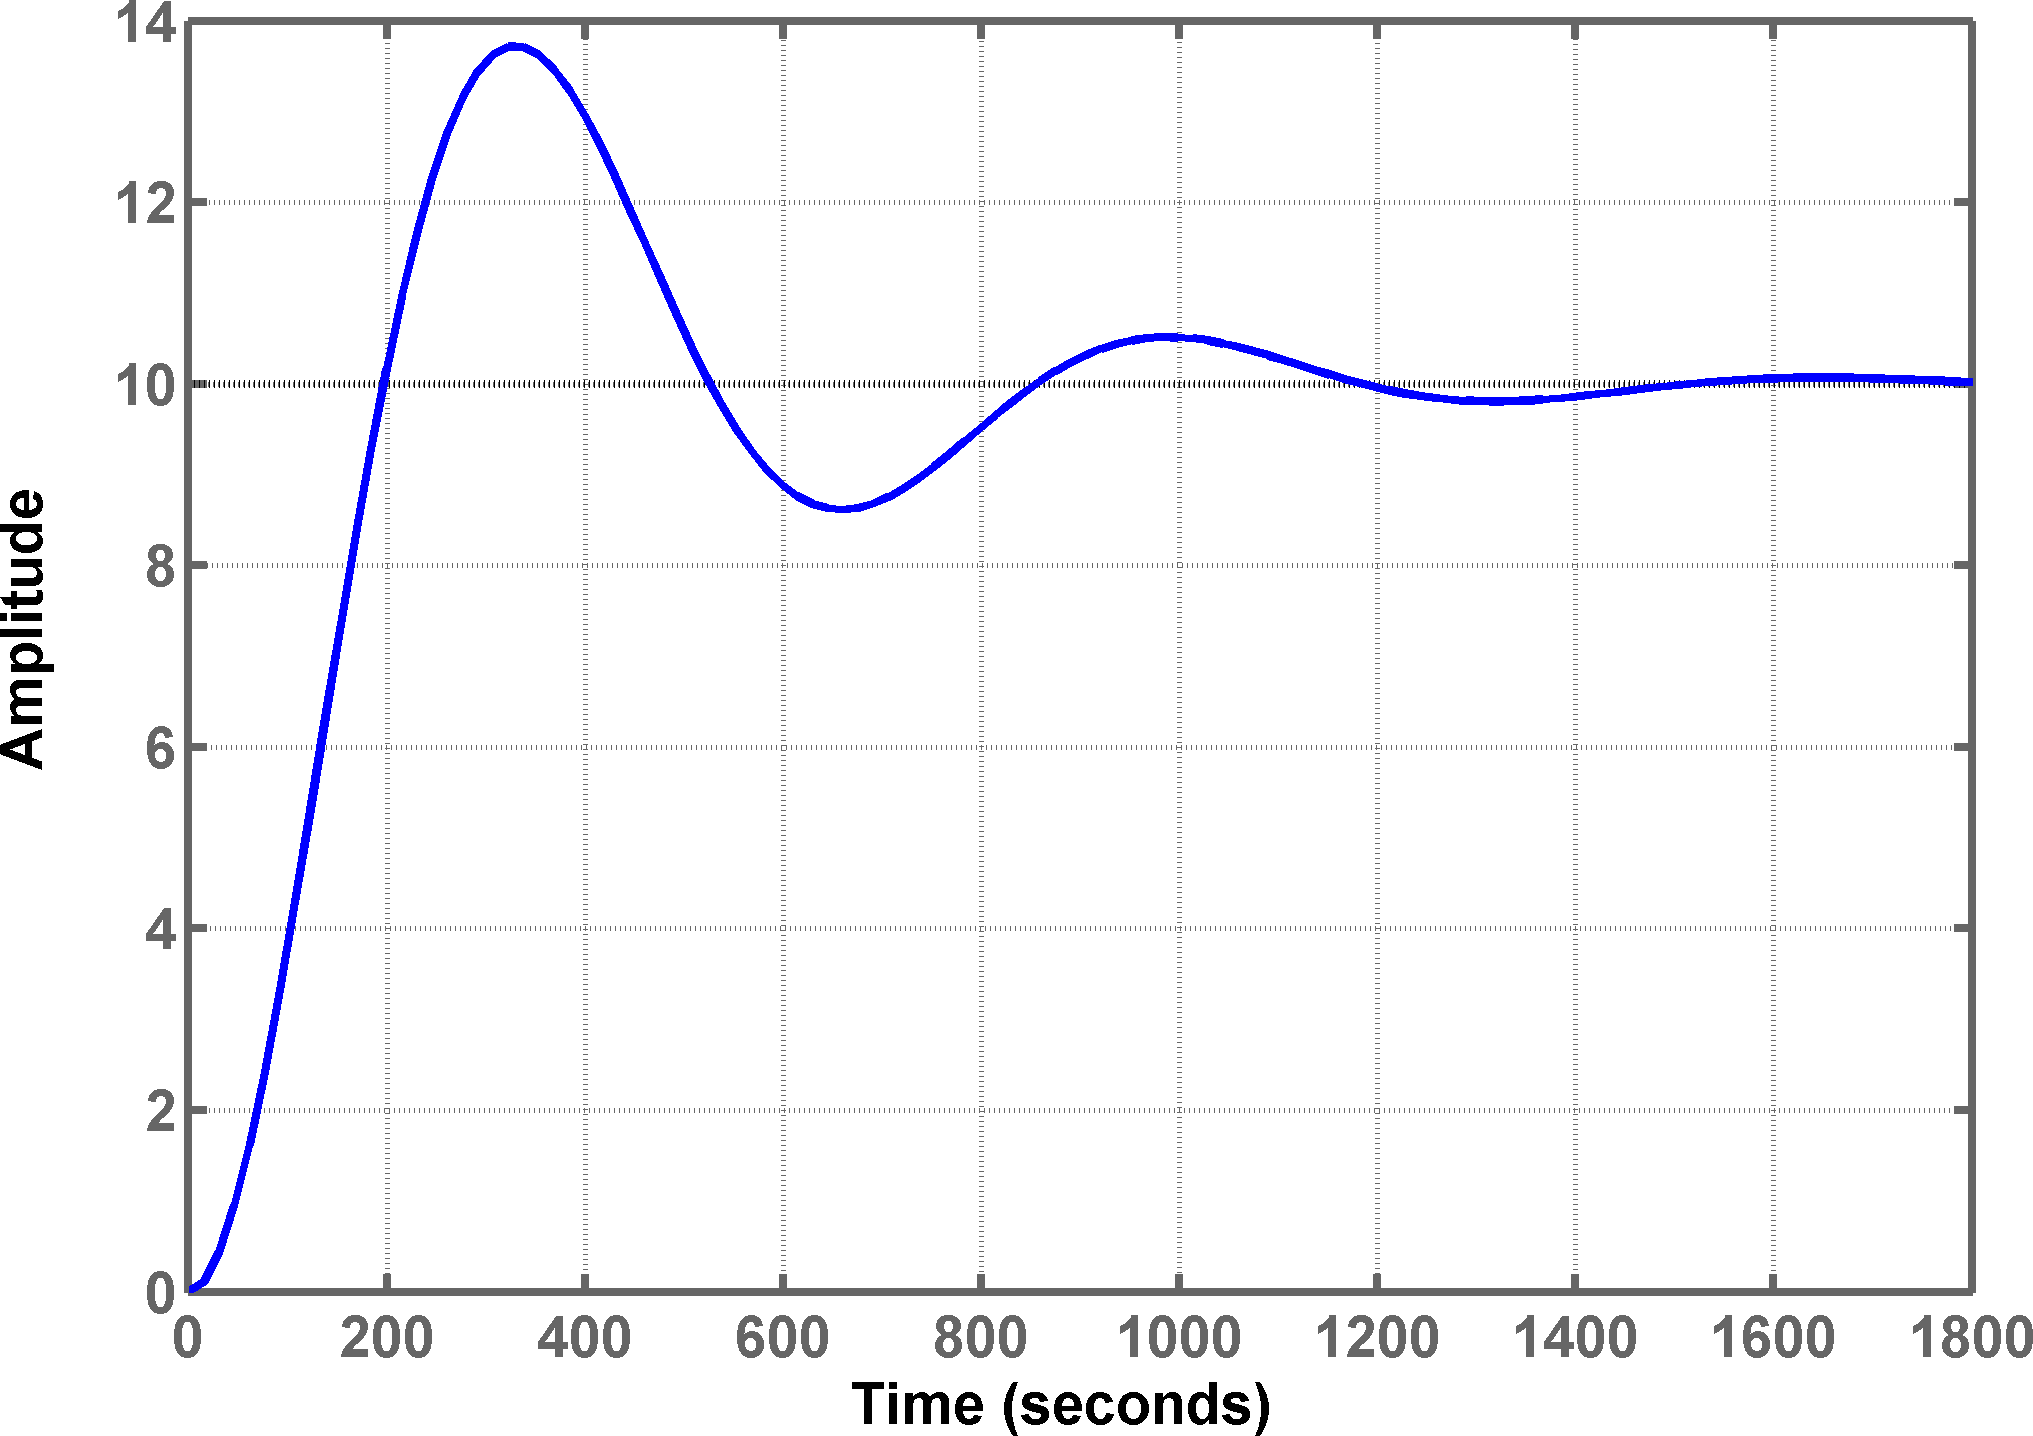
\includegraphics[width=0.5\linewidth]{images/general/step_pt2}
\end{center}
\caption{Step response of a $PT_2$ element}
\label{fig:step_pt2}
\end{figure}
TODO: step of pt1!!

Using the turn tangent principle depicted in Figure \ref{fig:wendetangentenverfahren}, the parameters $T_u$, $T_g$ and $K_s$ can be derived from the step response.

\begin{figure}[H]
\begin{center}
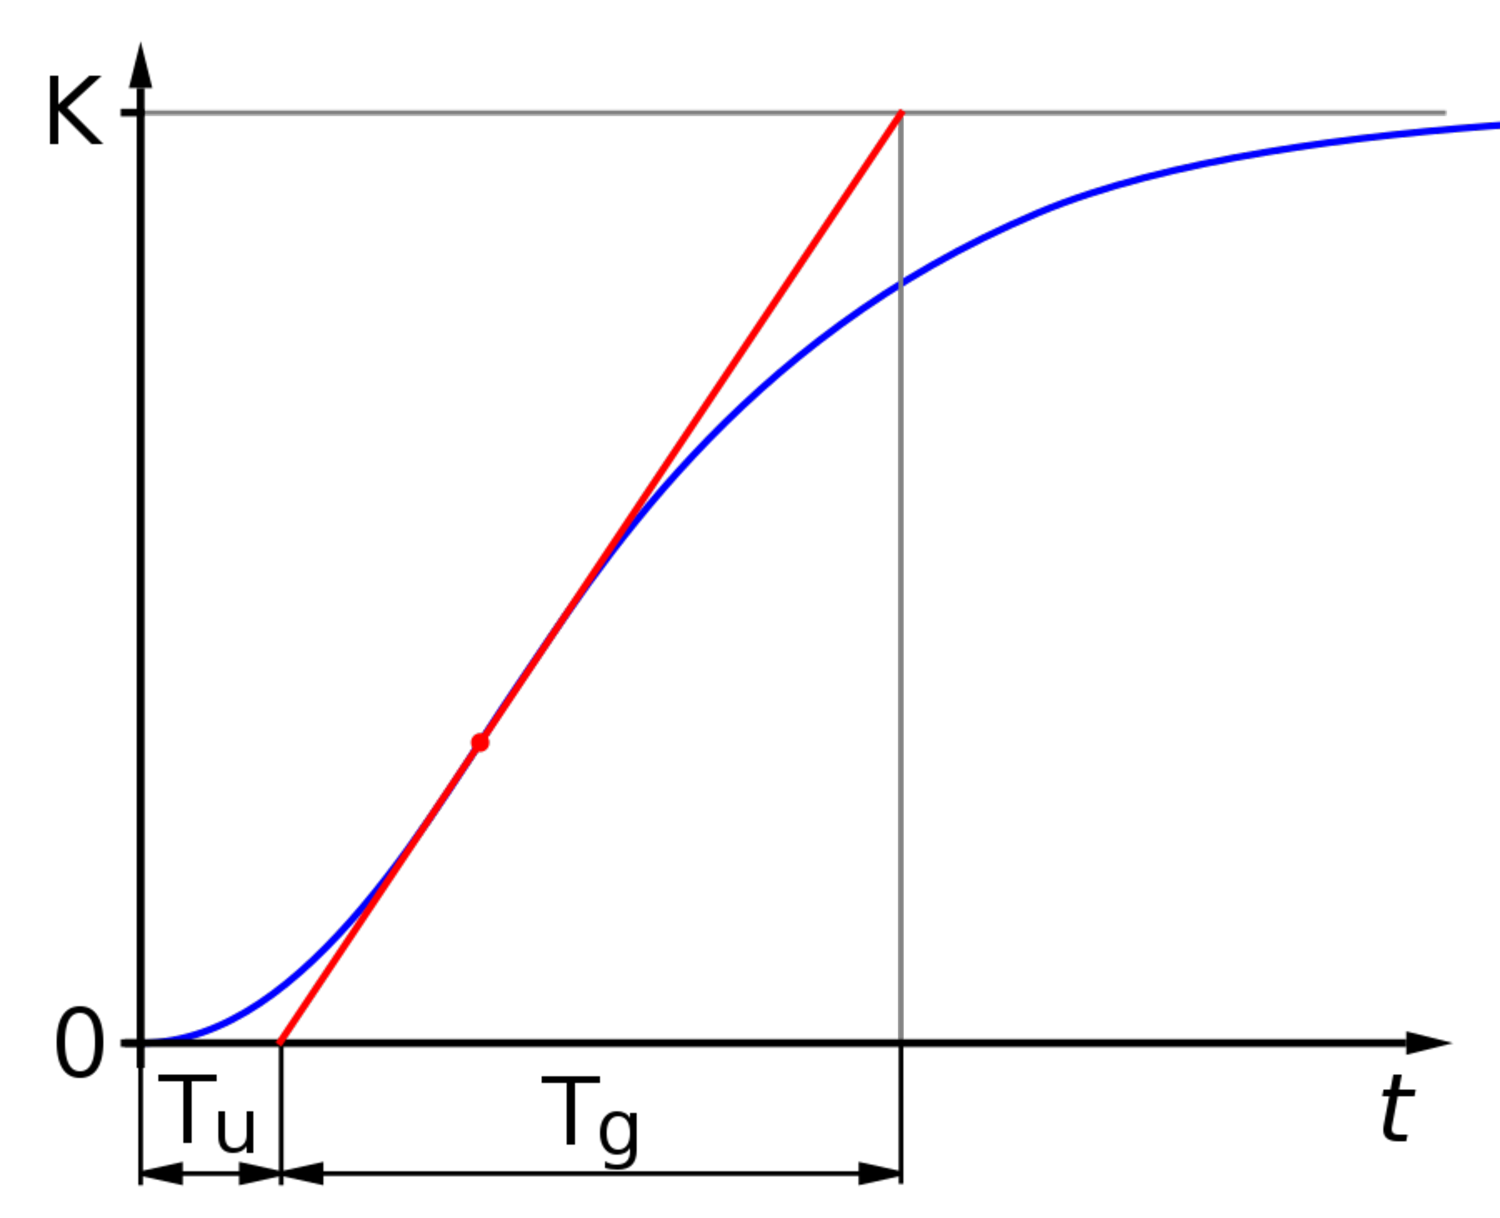
\includegraphics[width=0.5\linewidth]{images/general/wendetangentenverfahren}
\end{center}
\caption{Turn Tangent Principle}
\label{fig:wendetangentenverfahren}
\end{figure}

Once those paramters are known, the PID parameters can be calculated as formulated in Table \ref{tab:chien}.

\begin{table}[H]
\begin{center}
\begin{tabular}{ l | c | c | c}
  Controller Type & $K_p$ & $T_i$ & $T_d$\\
  \hline
  \hline
  P & $0.3 * \frac{T_g}{T_u * K_s}$& - & -\\
  \hline
  PI & $0.35 * \frac{T_g}{T_u * K_s}$ & $1.2 * T_g$ & - \\
  \hline
  PID & $0.6 * \frac{T_g}{T_u * K_s}$ & $T_g$ & $0.5 * T_u$\\
  \hline
\end{tabular}
\end{center}
\caption{Chien, Hrones, Reswick Method}
\label{tab:chien}
\end{table}

\subsubsection{Ziegler-Nichols}
\label{subs:Ziegler-Nichols}

To use this also called oscillation method the system characteristics are determined by bringing the system to the brink of oscillationby increasing $K_p$ whilst the I and D parts remain zero. The parameters $K_u$ and $T_u$ are then the gain $K_p$ and the period of the oscillating output.

The PID parameters then can be calculated according to Table \ref{tab:ziegler}.

\begin{table}[H]
\begin{center}
\begin{tabular}{ l | c | c | c}
  Controller Type & $K_p$ & $T_i$ & $T_d$\\
  \hline
  \hline
  P & $0.5 * K_{P.crit}$& - & -\\
  \hline
  PI & $0.45 * K_{P.crit}$ & $0.85 * \tau_{crit}$ & - \\
  \hline
  PID & $0.6 * K_{P.crit}$ & $0.5 * \tau_{crit}$ & $0.12 * \tau_{crit}$\\
  \hline
\end{tabular}
\end{center}
\caption{Ziegler-Nichols Method}
\label{tab:ziegler}
\end{table}
